\documentclass[12pt]{article}
%\usepackage[english]{babel}
%\usepackage[utf8x]{inputenc}
\usepackage{fullpage}
\usepackage{float}
\usepackage{booktabs}

\usepackage{listings}
\usepackage{color}

\title{Supplemental Information}
\author{Pedersen \textit{et al.}}

\date{}

\definecolor{mygreen}{rgb}{0,0.6,0}
\definecolor{mygray}{rgb}{0.5,0.5,0.5}
\definecolor{mymauve}{rgb}{0.58,0,0.82}

\lstset{ %
  backgroundcolor=\color{white},   % choose the background color
  basicstyle=\footnotesize,        % size of fonts used for the code
  breaklines=true,                 % automatic line breaking only at whitespace
  captionpos=b,                    % sets the caption-position to bottom
  commentstyle=\color{mygreen},    % comment style
  escapeinside={\%*}{*)},          % if you want to add LaTeX within your code
  keywordstyle=\color{blue},       % keyword style
  stringstyle=\color{mymauve},     % string literal style
}
\usepackage{graphicx}

\begin{document}

\maketitle

\section{Advantages}
\textit{bwa-meth} provides a number of advantages:

1. ease of use -- a single script indexes the fasta, aligns the reads, and
   tabulates methylation. Default parameters work well.

2. speed -- due to the efficient parallelization by bwa, bwa-meth can run on
   as many CPU's are available on a single machine.

3. disk-usage -- bwa-meth can take either compressed or uncompressed files
   and the reads are streamed directly to the aligner, never written to disk. An
   aligner that requires trimmed reads and that writes the converted reads to
   disk will require 3X as much storage for just the raw sequence data.

4. useful output -- the BAM that results from bwa-meth is sorted, indexed and
   contains the proper mapping quality scores, alignment flags, and read-groups.
   In addition, the header @SQ lines are sorted so that tools like Picard and
   GATK will accept them as is.

5. simplicity -- we have carefully designed bwa-meth to be quite simple and
   the code readable so that enhancements are simple. For example, see \#6.

6. strand-specificity -- Devon Ryan,
   the author of Bison, noted that many capture methods target only the reverse
   strand -- commonly called the original bottom. Though this would be simple to
   add to any aligner, ours is the only one that currently supports this. See
   from the supplemental figure 5 for the reduction in off-target reads that results
   from only considering reads that align to the original bottom strand.

7. specificity and sensitivity -- while the difference between aligners in
   this regard is small, we have shown that bwa-meth consistently performs as
   the best or among the best. We believe this to be the case in general and
   not limited to the specific cases that we have shown.

8. accuracy without trimming -- the accuracy is due in part to bwa's local
   alignment. This is something that is not supported in bismark and means that
   we can achieve very good accuracy without performing additional trimming
   which would result in additional disk-usage and processing time.


\section{Aligners Compared}

\begin{table}[!htp]
\caption{Methods Compared}
{\begin{tabular}{lll}\\\toprule
software & version & arguments\\\midrule
bismark (bowtie1) & 0.11.1 & --gzip --bam -n 2 -l 24\\
bismark (bowtie2) & 0.11.1 & --gzip --bam -N 1 --score\_min L,-0.4,-0.5\\ 
bsmap & 2.74 & bsmap -v3 -m0 -x1000 -S42 -n0 -s12 -I1\\
bsmooth & fb3f7ef & --very-sensitive\\
bison & 0.3.0 & --directional --very-sensitive-local -N 1\\
bwa-meth & 0.10 & bwa-meth\\
gsnap & 2014-02-28 & --npaths 1 --quiet-if-excessive -k 15\\
last & 392 & last-bisulfite-paired.sh\\\bottomrule
\end{tabular}}
\end{table}
We used a modified version of the calling script for last available in the
github repository.

\section{Comparison On Real Data}

We compared 7 aligners on real data as described in the text. Supplemental
Figure 1 below shows the same data as Figure 1 from the main text.

\begin{figure}[H]%supplemental figure1
    \centerline{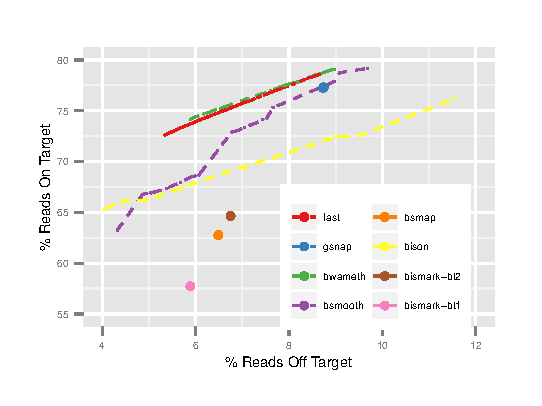
\includegraphics[width=125mm]{real-quals.eps}}
    \caption{Percent of paired-end, 100-base reads on (y) and off (x) target for
    the tested aligners. Aligners that report mapping quality are shown as lines
that span each quality cut-off. Reads are limited to those considered as primary, mapped alignments by the aligner. This is a color version of figure 1 from the paper}\label{suppfig:01}
\end{figure}

When we trim the reads with \emph{trim\_galore} before aligning, the result is shown below in Supplemental Figure 2. We report the percent of reads aligned relative
to the original count in the untrimmed data because we are interested in the
overall mapping rate.

%\begin{figure}[!htpb]%figure2
\begin{figure}[H]%figure2
    \centerline{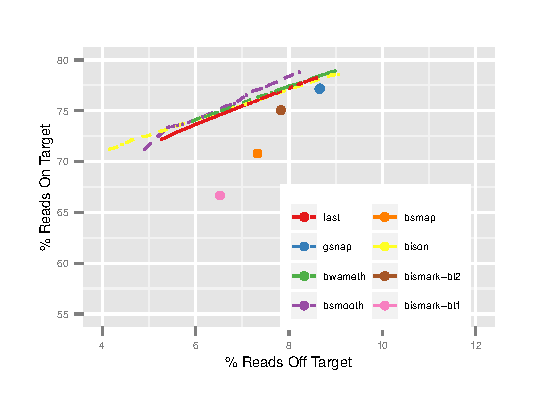
\includegraphics[width=125mm]{real-trim-quals.eps}}
    \caption{Percent of paired-end, \emph{trimmed} 100-base reads on (y) and off (x) target for the tested aligners. Aligners that report mapping quality are shown as connected dots for each quality cut-off. Reads are limited to those considered as primary, mapped alignments by the aligner.}\label{suppfig:02}
\end{figure}

\subsection{Resources}

%http://truben.no/latex/table/
\begin{table}[H]
    \centering
    \caption{Resources on real data}
    \begin{tabular}{lllll} \hline
    trimmed & program & CPU time(min) & mem(GB) & dataset \\ \hline

no &    bis1 & 588.68 & 8.30 & real \\
no &    bis2 & 2067.23 & 9.88 & real \\
no &    bison & 1639.25 & 10.34 & real \\
no &    bsmap & 8498.52 & 23.06 & real \\
no &    bsmooth & 5469.96 & 9.94 & real \\
no &    bwa & 490.37 & 17.70 & real \\
no &    gsnap & 5309.48 & 12.73 & real \\
no &    last & 611.22 & 34.53 & real \\

yes &    bis1 & 581.60 & 8.28 & real \\
yes &    bis2 & 1921.00 & 9.64 & real \\
yes &    bison & 1433.06 & 10.06 & real \\
yes &    bsmap & 7259.29 & 23.19 & real \\
yes &    bsmooth & 5189.16 & 9.46 & real \\
yes &    bwa & 413.69 & 17.65 & real \\
yes &    gsnap & 4565.57 & 13.93 & real \\
yes &    last & 560.53 & 34.53 & real \\

    \end{tabular}
\end{table}

\section{Comparison On Simulated Data}
Paired-end, 100-base reads were simulated using the tool \emph{Sherman}
(http://www.bioinformatics.babraham.ac.uk/projects/sherman/) with 95\% of the
reads simulated from mm10 and 5\% of the reads from \emph{E. coli}. 
Reads were aligned with the parameters in Supplemental Table 1.
Reads from \emph{E. coli} aligning to \emph{mm10} were considered as
off-target reads. The Y-axis in the plot is the percent of the \emph{mm10}
reads. Exact parameters sent to Sherman are here:
https://github.com/brentp/bwa-meth/blob/master/compare/src/gen-simulated.sh

Note that these reads have no insertions or deletions. We simulated the 
\emph{E. coli} reads to be 98\% unmethylated and we used a per-base error
rate of 1\% for the simulations.

Supplemental Figure 3 below shows the result for these simulations.

\begin{figure}[H]%figure3
    \centerline{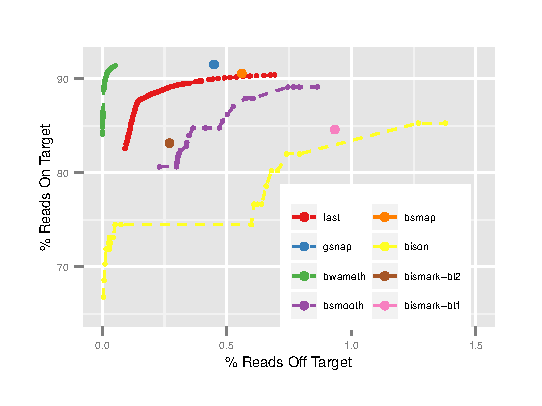
\includegraphics[width=125mm]{sim-quals.eps}}
    \caption{Percent of paired-end, \emph{simulated} 100-base reads on (y) and off (x)
    target for the tested aligners. Aligners that report mapping quality are shown as
    connected dots for each quality cut-off. Reads are limited to those considered as
    primary, mapped alignments by the aligner.
}\label{suppfig:03}
\end{figure}

Supplemental Figure 4 below shows the result for trimmed and simulated reads.
Trimming removes some read-pairs if one or both reads had low-quality. We
report the percent of reads aligned relative to the original, 
un-trimmed number from \emph{mm10} since we are interested in the overall
mapping rate.

\begin{figure}[H]%figure3
    \centerline{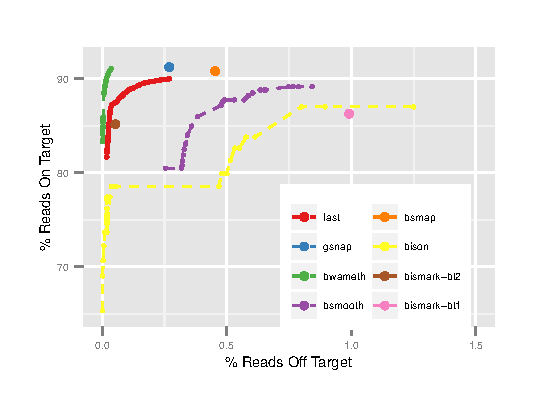
\includegraphics[width=125mm]{sim-trim-quals.eps}}
    \caption{Percent of paired-end, \emph{trimmed}, \emph{simulated} 100-base reads on (y) and off (x) target for the tested aligners. Aligners that report mapping quality are shown as connected dots for each quality cut-off. Reads are limited to those considered as primary, mapped alignments by the aligner.
}\label{suppfig:04}
\end{figure}

\subsection{Resources}

%http://truben.no/latex/table/
\begin{table}[H]
    \centering
    \caption{Resources on simulated data with 1\% error-rate
(programs run with more processes will use more memory)}
    \begin{tabular}{lllll} \hline
    trimmed & program & CPU time(min) & mem(GB) & dataset \\ \hline

no &    bis1 & 69.07 & 8.28 & sim \\
no &    bis2 & 271.13 & 9.66 & sim \\
no &    bison & 222.23 & 9.51 & sim \\
no &    bsmap & 227.35 & 22.99 & sim \\
no &    bsmooth & 501.97 & 9.52 & sim \\
no &    bwa & 145.56 & 19.40 & sim \\
no &    gsnap & 265.41 & 10.84 & sim \\
no &    last & 138.50 & 25.90 & sim \\

yes &    bis1 & 62.92 & 8.27 & sim \\
yes &    bis2 & 227.30 & 9.47 & sim \\
yes &    bison & 154.81 & 9.16 & sim \\
yes &    bsmap & 93.70 & 22.84 & sim \\
yes &    bsmooth & 461.71 & 9.31 & sim \\
yes &    bwa & 199.15 & 22.25 & sim \\
yes &    gsnap & 91.98 & 10.78 & sim \\
yes &    last & 113.80 & 25.90 & sim \\


    \end{tabular}
\end{table}

\section{Comparison On Error-Free Simulated Data}

Paired-end, error-free 100-base reads were simulated as above but
without contamination or errors.
Exact parameters sent to Sherman are here:
https://github.com/brentp/bwa-meth/blob/master/compare/src/gen-simulated.sh

Supplemental Figure 5 below shows the result for these simulations.
    
\begin{figure}[H]%figure5
    \centerline{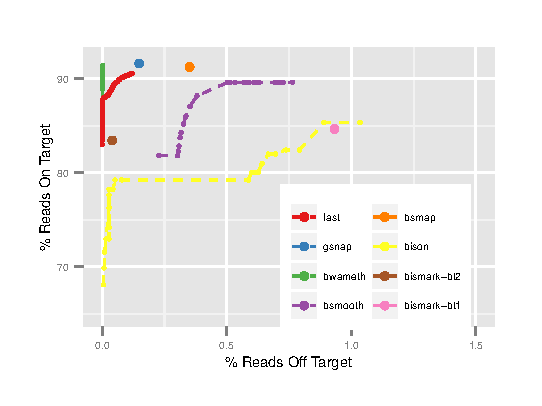
\includegraphics[width=125mm]{noerrorsim-quals.eps}}
    \caption{Percent of paired-end, \emph{error-free, simulated} 100-base reads on (y) and off (x)
    target for the tested aligners. Aligners that report mapping quality are shown as
    connected dots for each quality cut-off. Reads are limited to those considered as
    primary, mapped alignments by the aligner.
}\label{suppfig:05}
\end{figure}

Supplemental Figure 6 below shows the result for trimmed and simulated reads.
Trimming removes some read-pairs if one or both reads had low-quality. We
report the percent of reads aligned relative to the original, 
un-trimmed number from \emph{mm10} since we are interested in the overall
mapping rate. 
 
\begin{figure}[H]%figure6
    \centerline{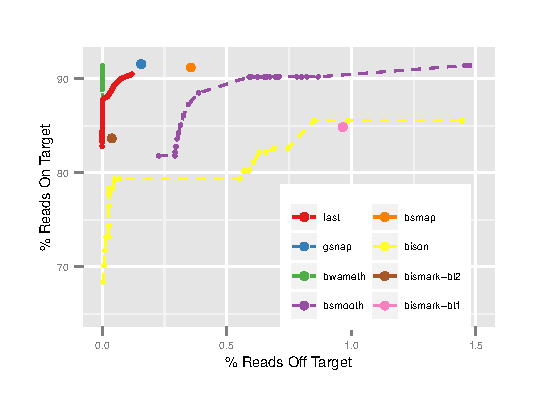
\includegraphics[width=125mm]{noerrorsim-trim-quals.eps}}
    \caption{Percent of paired-end, \emph{trimmed}, \emph{error-free, simulated} 100-base reads on (y) and off (x) target for the tested aligners. Aligners that report mapping quality are shown as connected dots for each quality cut-off. Reads are limited to those considered as primary, mapped alignments by the aligner.
}\label{suppfig:06}
\end{figure}



\subsection{Resources}

%http://truben.no/latex/table/
\begin{table}[H]
    \centering
    \caption{Resources on error-free simulated data
(programs run with more processes will use more memory)}
    \begin{tabular}{lllll} \hline
    trimmed & program & CPU time(min) & mem(GB) & dataset \\ \hline

no &    bis1 & 61.05 & 8.27 & error-free \\
no &    bis2 & 289.67 & 9.46 & error-free \\
no &    bison & 179.17 & 9.27 & error-free \\
no &    bsmap & 66.03 & 22.72 & error-free \\
no &    bsmooth & 492.62 & 9.37 & error-free \\
no &    bwa & 170.66 & 21.11 & error-free \\
no &    gsnap & 48.36 & 10.25 & error-free \\
no &    last & 214.68 & 25.90 & error-free \\

yes &    bis1 & 64.32 & 8.27 & error-free \\
yes &    bis2 & 245.42 & 9.48 & error-free \\
yes &    bison & 184.55 & 9.10 & error-free \\
yes &    bsmap & 67.68 & 22.94 & error-free \\
yes &    bsmooth & 481.99 & 9.38 & error-free \\
yes &    bwa & 173.93 & 21.43 & error-free \\
yes &    gsnap & 51.11 & 11.69 & error-free \\
yes &    last & 138.03 & 25.90 & error-free \\

    \end{tabular}
\end{table}



\section{Improved Accuracy for Stranded Capture Experiments}

Below we show a reduction in the percent of off-target reads by
considering only the strand targetted by our capture protocol.

\begin{figure}[H]%figure7
    \centerline{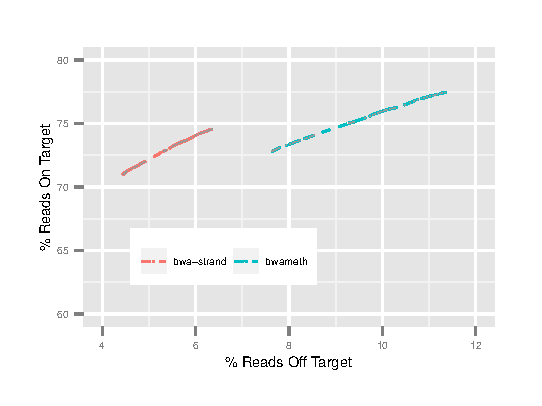
\includegraphics[width=86mm]{real-bwa-strand.eps}}
    \caption{For a capture experiment that targets only one strand, we can
    improve accuracy by considering only reads that map to that strand.
    Here, we show the effect from the original bwameth alignments as shown
    in Figure 1 compared to the alignments restricted to the strand targeted
    by the capture method.}\label{suppfig:07}
\end{figure}

This is implemented in \textit{bwa-meth} via the \emph{--set-as-failed}
flag so that reads mapping to a given strand are given the SAM flag
indicating that they failed vendor quality control checks. Invocation
would look like this:

\begin{lstlisting}[language=bash]
bwameth.py \
    --reference $REF \
    --set-as-failed f \
    $READS_R1 $READS_R2

\end{lstlisting}
to set reads mapping to the forward, or original top strand
as failed.


\section{Mapping and Trimming}
We note that trimming improves accuracy for most aligners but the
difference is very small for \textit{bwa-meth}.

\section{\textit{bwa-meth} Installation And Requirements}

\textit{Bwa-meth} depends on samtools and a single python library, \textit{toolshed}.
The latter can be installed by running \emph{sudo python setup.py install} from the main
directory of the \textit{bwa-meth} project. Samtools is a C library installed on most
systems and available at https://github.com/samtools/samtools.
Further installation instructions are available in the \textit{bwa-meth} README at
https://github.com/brentp/bwa-meth/

For tabulation of methylation by CpG, \emph{Bis-SNP} \cite{bissnp} is required.
The java .jar file is available from: http://sourceforge.net/projects/bissnp/files/

For CNV detection from BS-Seq data, the R package \emph{cn.mops} \cite{cnmops} is required.
It is available
from bioconductor \cite{bioconductor} at: http://bioconductor.org/packages/devel/bioc/html/cn.mops.html
\section{Additional Features}
\textit{Bwa-meth} and GSNAP are the only programs that output a BAM file that passes picard's ValidateSam without errors.
Last does not report the proper pair information in all cases and none of the other aligners add a read-group.
For the comparison, we added sorting and forced SAM output by the other aligners regardless of their default.
\textit{Bwa-meth} outputs a read-group for each sample by default and allows that to be customized.

\textit{bwa-meth} can calculate bias of methylation estimates by location in the read:

\begin{lstlisting}[language=bash]
python bias-plot.py input.bam ref.fa
\end{lstlisting}
This will create a bias-plot showing bases in the reads that should not be considered
for methylation calls.

\textit{Bwa-meth} defers tabulation of the methylation scores to Bis-SNP \cite{bissnp} by offering a simplified interface:
\begin{lstlisting}[language=bash]
bwameth.py tabulate \
    --trim 3,3 \
    --map-q 30 \
    --bissnp BisSNP-0.82.2.jar \
     --reference /path/to/ref.fasta \
     input.bam
\end{lstlisting}
Where the arguments are sent to Bis-SNP to, for example trim the first and last 3 bases
from each read to avoid bias.

A full example on real data is at:
https://github.com/brentp/bwa-meth/tree/master/example/

%\begin{thebibliography}{}
\bibliographystyle{abbrv}
    \bibliography{document}
%\end{thebibliography}

\end{document}
